%October 2016, the 4th
\section{Lesson 3 - Hamming Space}

A space is a set that has structure. Consider the set of all binary strings $\{0, 1\}^*$; we can define a space with the distance metric. The \textbf{distance} is defined as a function $d: X \times X \rightarrow \mathbb{R}^+_0$. A metric has the following properties:
\begin{enumerate}
	\item \begin{enumerate}
		\item $d(x, y) \geq 0,\ \forall (x, y) \in X \times X$
		\item $d(x, y) = 0 \Leftrightarrow x = y$
	\end{enumerate}
	\item $d(x, y) = d(y, x), \forall (x, y) \in X \times X$
	\item $d(x, y) \leq d(x, z) + d(z, y)$
\end{enumerate}

What is the Hamming metric? Consider $\str{x}, \str{y}  \in \{0, 1\}^n$. Then the Hamming distance is defined as
\begin{equation}
	\hdist{x}{y} = |\{i\ |\ x_i \not= y_i\}|
\end{equation}

Why is it a metric? Consider $\str{x}$, $\str{y}$, $\str{z} \in \{0,1\}^n$. Then, with $D = \{i\ |\ x_i \not= y_i\}$ is true that 
\begin{center}
	\begin{math}i \in D \Rightarrow x_i \not=y_i \Rightarrow \neg (z_i = x_i \wedge z_i = y_i) \Rightarrow d_H(x_i, y_i) \leq d_H(z_i, x_i) + d_H(z_i, y_i).
	\end{math}
\end{center}

By the additive property we can write $$d_H(x, y) = \sum_{i = 1}^n d_H(x_i, y_i).$$ Summing up gives the triangle inequality.

If a string $\str{x}$ has been changed $r$ times to become $\str{y}$ then $d_H(\str{x}, \str{y}) \leq r$. Define a \textbf{Hamming ball} of radius $r$ around $\str{x}$ as 
$$B_H= \hball{x}{r} = \{\str{y}\ |\ \hdist{x}{y} \leq r\}.$$
Obviously $r$ needn't to be an integer (use the \emph{floor} function). Here are some properties of Hamming balls:
\begin{itemize}
	\item if one subtracts $\hball{x}{r}$ to $\{0, 1\}^n$ then the result is also an Hamming ball;
	\item $\{0, 1\}^n = \hball{x}{n},\ \forall \str{x} \in \{0, 1\}^n$, but if $r < n$ then the center is unique;
\end{itemize}

What we can say about $\hball{x}{r}$? For simplicity sake, consider $\hball{0}{r}$. Then the following holds:
\begin{equation}\label{eq:volume}
	|\hball{0}{r}| = \sum_{i = 0}^{\lfloor r \rfloor} \binom{n}{i}
\end{equation}

That is the number of ways in which we can flip to 1 the bits. From this follows that $\hdist{0}{y} + \hdist{1}{y} = n$.

We define the Hamming weight as $\hweight{x} = \hdist{0}{x}$. The following holds:
$$\str{y} \in \hball{0}{r} \Rightarrow \hweight{y} > r \Rightarrow \hdist{y}{1} < n - r \leq n -r - 1.$$

So it is true that

$$\overline{\hball{0}{n}} = \hball{1}{r'} = \hball{1}{n - r - 1}.$$

In other words the Hamming space can be partitioned into two Hamming balls. If $n$ is odd an Hamming space can be partitioned in the following way: $$\{0, 1\}^n = \hball{0}{\lfloor \dfrac{n}{2}\rfloor } \cup \hball{1}{\lfloor \dfrac{n}{2}\rfloor}$$
The Hamming space cannot be partitioned into three balls. In how many balls can $\{0, 1\}^n$ be partitioned? It cannot partitioned be partititoned into $s$ balls with $3 \leq s \leq n + 1$.

\subsection{The volume of an Hamming ball}
We have seen that the volume of a generic Hamming ball is described by equation \ref{eq:volume}. We can use the Pascal triangle to get a feeling about the order of magnitude of the Hamming ball. Consider the $n$th row in the triangle; since it is symmetric, if we split the row in half the sum of the terms of the first part is equal to the sum of the terms of the second part of the row. The volume of the greatest ball is $|\hball{0}{n}| = 2^n$; instead, the volume of the ball with radius $n/2$ (in the triangle's point of split) is $2^n/2 = 2^n2^{-1} = 2^{n-1}$. So, if $r \geq n/2$ then $2^{n-1} \leq |\hball{0}{r}| \leq 2^n$. Can we bound the volume for $r < n/2$?

First we introduce the notion of \textbf{entropy}, a function $h: [0, 1] \rightarrow [0, 1]$ defined as follows:
\begin{center}
	$h(t) = t\log_2(\dfrac{1}{t}) + (1 - t)\log_2\left(\dfrac{1}{1-t}\right)$
\end{center}

The plot of $h$ looks like this:
\begin{figure}[h]
	\centering
	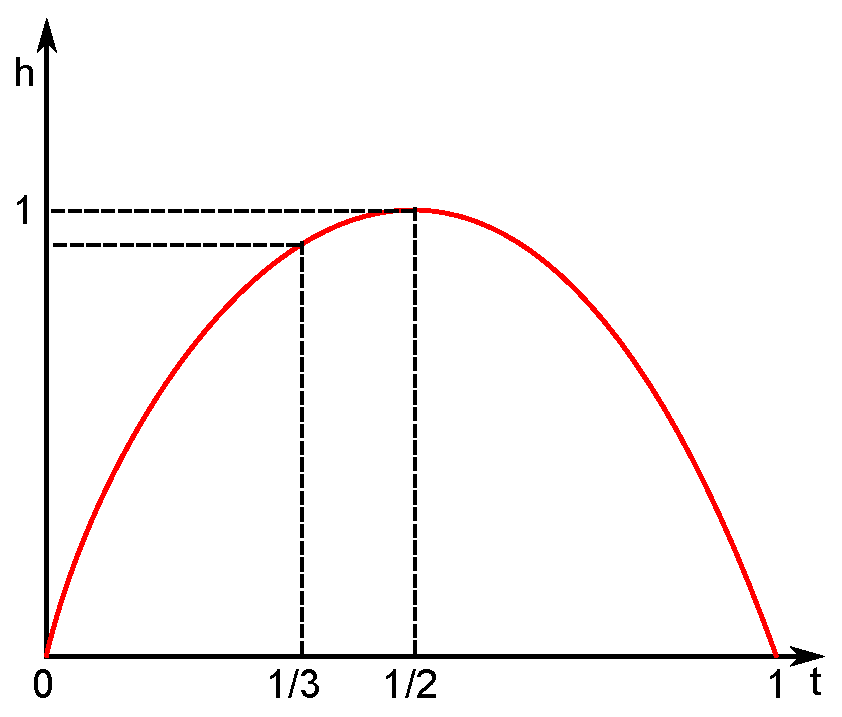
\includegraphics[width=210px]{pictures/ch01-i00.eps}
	\caption{The entropy function.}
\end{figure}

This function is not defined for the values $0$ and $1$ but we have limits defined on these points, and they are both $0$. So we artificially set $h(0) = 0$ and $h(1) = 0$. It is better to think about it as probability distribution $(t, 1 - t)$ and entropy is a number attached to it. Entropy measures symmetry and with $t = 1/2$ we have maximum chaos (the future outcomes are equally likely).